\chapter{Metodologia Proposta}
\label{chap4}


Este capítulo descreve a metodologia adotada para o desenvolvimento, avaliação e comparação dos modelos preditivos aplicados ao sistema de destilação por membranas estudado. A abordagem proposta integra etapas de preparação e estruturação dos dados experimentais, definição de estratégias de validação consistentes com a natureza dos dados, seleção e ajuste de modelos de diferentes níveis de complexidade e incorporação de informações provenientes de um modelo físico reduzido.

Inicialmente, são apresentados os procedimentos de organização do conjunto de dados, pré-processamento e engenharia de atributos, incluindo critérios baseados em fundamentos físicos para definição das variáveis de entrada. Em seguida, descrevem-se as estratégias de validação cruzada e os critérios adotados para estimação de desempenho e seleção de modelos, com ênfase no controle de sobreajuste e na consideração da incerteza associada às estimativas.

Posteriormente, é detalhada a estrutura computacional do \textit{pipeline} de modelagem, que será explicado em mais detalhes nas próximas seções, bem como as famílias de modelos avaliadas e os respectivos espaços de busca de hiperparâmetros. Por fim, são apresentadas as estratégias de integração entre o modelo físico e os modelos baseados em dados, estabelecendo o arcabouço metodológico que sustenta a análise comparativa desenvolvida neste trabalho.

\subsection{Síntese do pipeline metodológico}

\begin{figure}[H]
\centering
\resizebox{0.85\textwidth}{!}{%
\begin{tikzpicture}[
    node distance=0.9cm,
    every node/.style={font=\small},
    block/.style={
        rectangle,
        rounded corners,
        draw=black,
        thick,
        align=center,
        minimum width=5.6cm,
        minimum height=1.0cm,
        fill=gray!10
    },
    decision/.style={
        rectangle,
        rounded corners,
        draw=black,
        thick,
        align=center,
        minimum width=6.2cm,
        minimum height=1.1cm,
        fill=blue!8
    },
    smallblock/.style={
        rectangle,
        rounded corners,
        draw=black,
        thick,
        align=center,
        minimum width=5.2cm,
        minimum height=0.9cm,
        fill=gray!8
    },
    arrow/.style={->, thick}
]

\node[block] (data)
{Dados experimentais};

\node[block, below=of data] (eda)
{Análise exploratória dos dados\\
e análise de correlação};

\node[block, below=of eda] (model0d)
{Avaliação do modelo físico reduzido (0D)\\
como referência teórica};

\node[decision, below=of model0d] (prep)
{Definição do pipeline de preparação dos dados};

\node[smallblock, below=of prep] (p1)
{Pipeline adotado: dados sem tratamento};

\node[block, below=of p1] (models)
{Seleção e comparação de famílias de modelos};

\node[smallblock, below=0.4cm of models] (families)
{OLS, Ridge, Lasso, ElasticNet, DT, RF, GB, MLP e modelos híbridos};

\node[block, below=of families] (cv)
{Validação cruzada por grupos (GroupKFold)\\
e critério de seleção: regra 1-SE + complexidade};

\node[block, below=of cv] (best)
{Análise detalhada do modelo vencedor};

\node[decision, below=of best] (final)
{Comparação final entre o modelo vencedor\\
e o modelo físico 0D};

\draw[arrow] (data) -- (eda);
\draw[arrow] (eda) -- (model0d);
\draw[arrow] (model0d) -- (prep);
\draw[arrow] (prep) -- (p1);
\draw[arrow] (p1) -- (models);
\draw[arrow] (models) -- (families);
\draw[arrow] (families) -- (cv);
\draw[arrow] (cv) -- (best);
\draw[arrow] (best) -- (final);

\end{tikzpicture}
}
\caption[Fluxograma do procedimento metodológico]{Fluxograma do procedimento metodológico adotado neste trabalho, desde a análise exploratória dos dados experimentais até a comparação final entre o modelo baseado em dados selecionado e o modelo físico reduzido (0D). O diagrama evidencia as principais etapas do estudo, incluindo a definição do procedimento de preparação dos dados, a avaliação de diferentes famílias de modelos e a seleção do modelo final com base em critérios de desempenho e parcimônia. Fonte: Autor.}
\label{fig:fluxograma_resultados_pipeline}
\end{figure}

\section{Estrutura do Sistema e Preparação dos Dados}
\label{sec:estrutura_sistema_dados}

Antes da construção dos modelos preditivos, é necessário delimitar o sistema físico que se deseja representar. Neste trabalho, considera-se um sistema de destilação por membranas na configuração \textit{Vacuum-Enhanced Air Gap Membrane Distillation} (V-AGMD), operado em escala piloto. O sistema utiliza um módulo espiralado, no qual a solução salina aquecida escoa pelos canais de alimentação, separados dos espaços de ar por membranas hidrofóbicas. Do outro lado do espaço de ar, placas de resfriamento atuam como superfícies de condensação, sendo mantidas frias pela circulação de água nos canais de resfriamento. A unidade também inclui um sistema de vácuo, responsável por induzir pressão reduzida no tanque de permeado e nos espaços de ar, além de um tanque para coleta do destilado (\cite{Lisboa2024}).

O funcionamento do processo está associado à diferença de temperatura entre a alimentação aquecida e a região fria de condensação. Essa diferença estabelece um gradiente de pressão parcial de vapor que promove a evaporação da água na interface entre a solução salina e a membrana. O vapor formado atravessa os poros da membrana hidrofóbica, enquanto os sais dissolvidos são retidos na alimentação. Em seguida, o vapor percorre o espaço de ar sob pressão reduzida e se difunde em direção à superfície fria de condensação, onde condensa e é coletado como permeado. A presença do espaço de ar contribui para reduzir perdas térmicas por condução, enquanto a operação sob vácuo reduz a resistência ao transporte de massa no domínio gasoso, favorecendo o aumento do fluxo de permeado (\cite{Lisboa2024}).

Do ponto de vista físico, o desempenho do sistema é governado pelo acoplamento entre transferência de massa e transferência de calor. A transferência de massa envolve o transporte de vapor através da membrana hidrofóbica e do espaço de ar, enquanto a transferência de calor inclui a convecção nas correntes líquidas, a condução através da membrana e do espaço de ar e o transporte de calor latente associado ao vapor. Dessa forma, alterações nas condições operacionais, como temperaturas de entrada, vazão, pressão de vácuo e salinidade, afetam diretamente a produtividade do processo e o comportamento térmico do módulo.

No presente trabalho, o sistema físico é representado por meio de variáveis operacionais de entrada e variáveis de desempenho de saída. As variáveis de entrada consideradas são a temperatura de entrada da alimentação, a temperatura de entrada da corrente de resfriamento, a vazão de entrada da corrente de resfriamento, a pressão de vácuo e a concentração de NaCl. Essas variáveis estão associadas à força motriz térmica do processo, ao regime de escoamento e tempo de residência das correntes, à resistência difusiva no espaço de ar e às propriedades termofísicas da solução salina. As variáveis de saída são o fluxo de permeado e as temperaturas de saída das correntes de alimentação e resfriamento.

A escolha dessas saídas está relacionada aos principais parâmetros de desempenho do sistema. O fluxo de permeado representa a produtividade do processo da destilação e, por isso, constitui a variável de maior interesse operacional neste trabalho. As temperaturas de saída, por sua vez, permitem avaliar o comportamento térmico do módulo e são relevantes para análises energéticas posteriores, incluindo a estimativa de indicadores como o consumo específico de energia térmica e a razão de ganho de saída. Dessa forma, os modelos avaliados neste trabalho buscam aprender a relação entre as condições operacionais impostas ao sistema V-AGMD e as respostas associadas tanto à produção de permeado quanto ao desempenho térmico do módulo.

\subsubsection{Estruturação do Conjunto de Dados}

O conjunto de dados utilizado neste trabalho é composto por observações experimentais associadas à operação de um sistema V-AGMD em escala piloto. Neste contexto, cada observação, ou ponto experimental, corresponde a uma linha da base de dados e representa uma condição específica de operação do módulo. Essa condição é definida pela combinação dos valores impostos às variáveis controladas experimentalmente: temperatura de entrada da alimentação, temperatura de entrada da corrente de resfriamento, vazão da corrente de resfriamento, pressão de vácuo no espaço de ar e concentração de NaCl. Essas variáveis descrevem as condições sob as quais o processo foi conduzido e estão diretamente relacionadas à força motriz térmica, ao regime de escoamento, à resistência difusiva no espaço de ar e às propriedades da solução salina (\cite{Lisboa2024}).

Para cada ponto experimental, foram registradas ou calculadas as respostas do sistema, isto é, as variáveis que caracterizam o desempenho do módulo naquela condição de operação. No contexto deste trabalho, as saídas consideradas são o fluxo de permeado e as temperaturas de saída das correntes de alimentação e de resfriamento. O fluxo de permeado representa a produtividade do processo, enquanto as temperaturas de saída permitem avaliar o comportamento térmico do módulo e servem como base para análises energéticas posteriores.

Dessa forma, a base de dados pode ser interpretada como uma tabela experimental estruturada para modelagem preditiva: cada linha corresponde a uma condição operacional testada no sistema V-AGMD, enquanto as colunas representam, de um lado, as variáveis de entrada controladas no experimento e, de outro, as respostas medidas ou calculadas para essa mesma condição.

Formalmente, o problema é estruturado como uma tarefa de regressão supervisionada de múltiplas saídas. Seja
\[
X \in \mathbb{R}^{n \times p}
\]
a matriz de variáveis de entrada, onde \( n \) representa o número total de observações experimentais e \( p \) o número de variáveis operacionais consideradas. Cada linha de \( X \) corresponde a um vetor de condições de operação do sistema.

As variáveis de saída são organizadas na matriz
\begin{equation}
Y \in \mathbb{R}^{n \times 3}    
\end{equation}

\noindent em que \(n\) representa o número total de observações experimentais e o número \(3\) corresponde às três variáveis de saída consideradas na modelagem.

cujas colunas representam, respectivamente, as temperaturas de saída do canal quente, as temperaturas de saída do canal frio e o fluxo de permeado. Dessa forma, cada observação experimental está associada simultaneamente a três grandezas de interesse, caracterizando o problema como regressão de multiplas saídas.

Além das matrizes \(X\) e \(Y\), a base de dados contém a variável denominada \textit{Regime}. Neste trabalho, o termo \textit{Regime} refere-se a um agrupamento de observações experimentais obtidas sob condições operacionais equivalentes ou próximas. Assim, amostras pertencentes ao mesmo regime compartilham características comuns do ensaio e, por isso, não devem ser tratadas como completamente independentes durante a avaliação dos modelos.

A variável \textit{Regime} é mantida separadamente das matrizes \(X\) e \(Y\), sendo utilizada exclusivamente para fins de agrupamento no processo de validação cruzada. Essa escolha permite preservar a estrutura dependente dos dados durante a etapa de avaliação de desempenho.

Essa organização formal estabelece a base para as etapas subsequentes de pré-processamento, validação e seleção de modelos.

\begin{figure}[H]
    \centering
    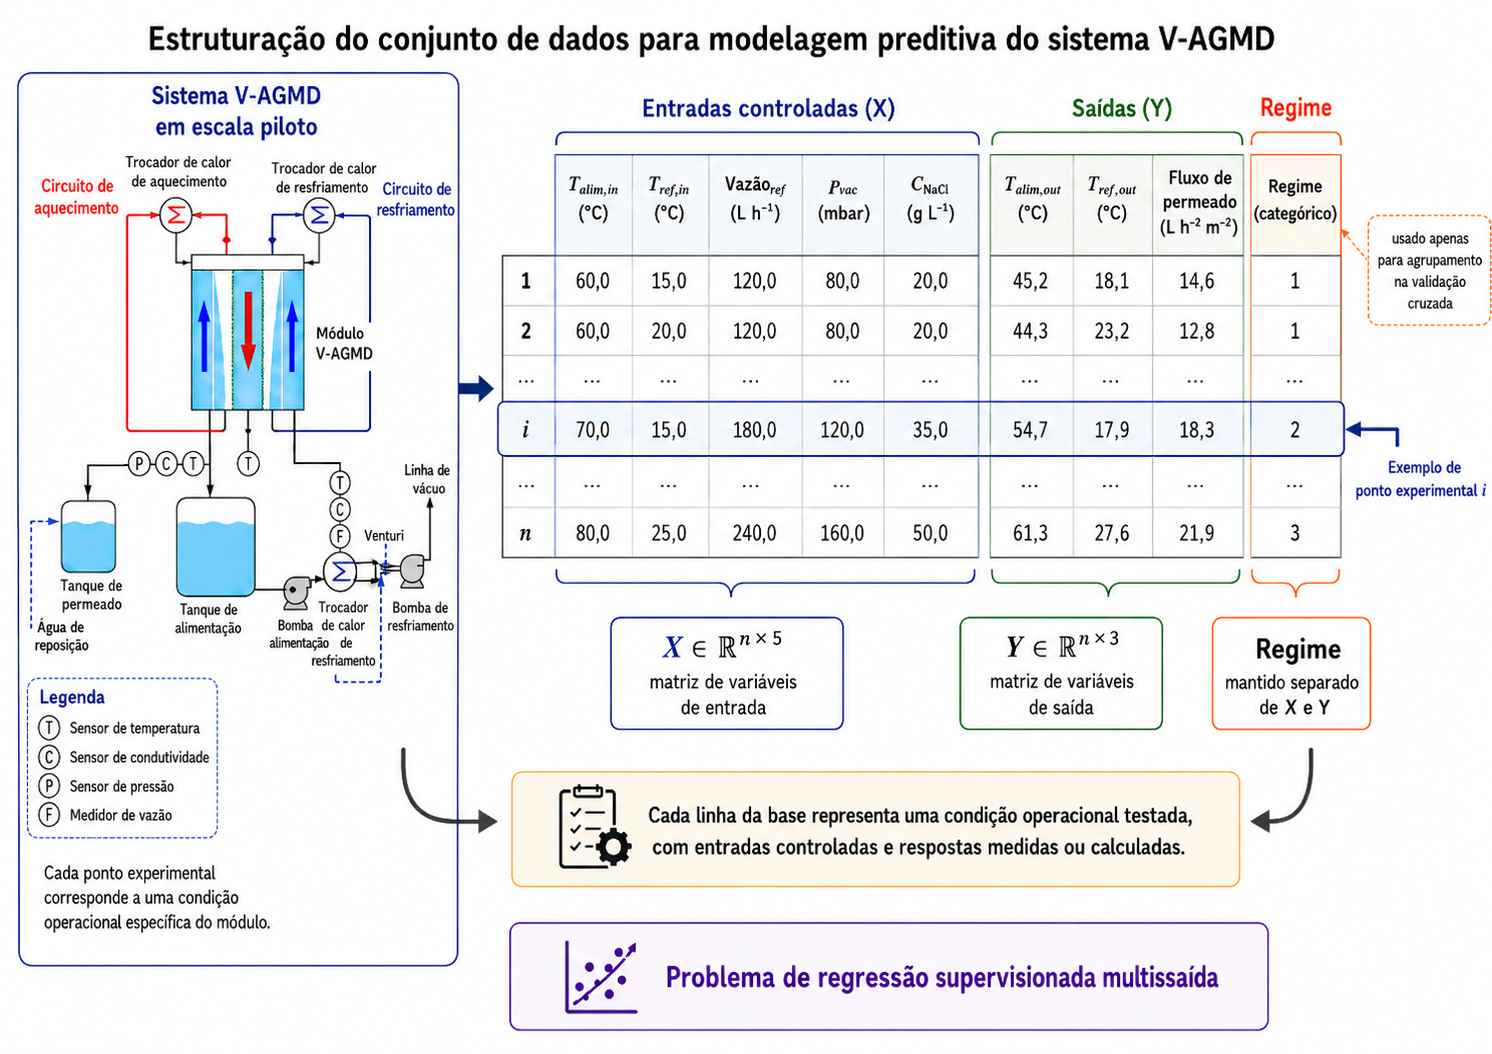
\includegraphics[width=1\linewidth]{Imagens/chap04/esquematizacao_regressao.png}
    \caption[Esquematização da estrutura do conjunto de dados para modelagem preditiva]{Esquematização da estrutura do conjunto de dados utilizado na modelagem preditiva do sistema V-AGMD. Cada linha da base representa um ponto experimental, definido por uma condição operacional específica do módulo. As variáveis de entrada são organizadas na matriz \(X \in \mathbb{R}^{n \times 5}\), enquanto as três variáveis de saída são organizadas na matriz \(Y \in \mathbb{R}^{n \times 3}\). A variável \textit{Regime} é mantida separadamente das matrizes \(X\) e \(Y\), sendo utilizada apenas para o agrupamento das observações na validação cruzada. Fonte: Elaborado pela autora com base em \cite{Lisboa2024}.}
    \label{fig:esquematizacao_regressao}
\end{figure}

\subsubsection{Tratamento da Variável de Agrupamento}

Como definido na seção anterior, a variável \textit{Regime} identifica grupos de observações experimentais associadas a condições operacionais equivalentes ou próximas. Essa variável não é utilizada como entrada dos modelos, mas apenas como informação auxiliar para orientar a divisão dos dados durante a validação cruzada.

A variável \textit{Regime} foi utilizada exclusivamente como identificador de agrupamento durante o processo de validação cruzada. Ela não foi incluída como variável de entrada nos modelos preditivos, a fim de evitar que o algoritmo explorasse informações implícitas sobre a estrutura experimental que não estariam disponíveis em cenários de generalização para novos regimes.

Essa decisão metodológica tem como objetivo preservar a coerência experimental do processo de avaliação. Caso observações pertencentes ao mesmo regime fossem distribuídas simultaneamente entre conjuntos de treinamento e validação, o modelo poderia se beneficiar de informações correlacionadas, produzindo estimativas excessivamente otimistas de desempenho.

Dessa forma, o particionamento dos dados foi conduzido respeitando os agrupamentos definidos pela variável \textit{Regime}, garantindo que todas as observações associadas a um mesmo regime fossem alocadas integralmente em um único subconjunto durante cada iteração da validação cruzada. Essa estratégia permite avaliar a capacidade dos modelos de generalizar para condições operacionais não previamente observadas.

\subsection{Estratégia de Escalonamento Adotada}

Neste trabalho, optou-se pela padronização das variáveis de entrada por meio da transformação para média zero e variância unitária, conforme definido pela Equação~\ref{eq:padronizacao_zscore}. Essa transformação corresponde ao procedimento implementado pelo \texttt{StandardScaler}, no qual cada variável é centralizada pela sua média e escalada pelo seu desvio padrão.

A escolha da padronização foi motivada pela presença de modelos lineares regularizados e redes neurais no conjunto de famílias avaliadas, ambos sensíveis à escala relativa das variáveis. Como este estudo tem como objetivo comparar diferentes classes de modelos sob um protocolo unificado de treinamento, validação e seleção, adotou-se uma única estratégia de escalonamento aplicável de forma consistente a todas as famílias. Dessa forma, reduz-se a influência arbitrária das unidades de medida sobre o desempenho dos modelos e torna-se mais justa a comparação entre abordagens distintas.


A transformação foi implementada por meio de um \textit{Pipeline}, isto é, uma sequência encadeada de etapas de pré-processamento e modelagem executadas de forma integrada. Nesse procedimento, o escalonamento não é aplicado previamente à base completa, mas sim incorporado ao fluxo de treinamento de cada modelo. Assim, em cada iteração da validação cruzada, o \texttt{StandardScaler} foi ajustado exclusivamente com os dados do subconjunto de treinamento, calculando a média e o desvio padrão apenas a partir dessas amostras. Em seguida, os mesmos parâmetros de padronização foram aplicados ao subconjunto de validação correspondente. Dessa forma, evitou-se o uso de estatísticas globais calculadas com o conjunto completo de dados, prevenindo vazamento de informação entre treino e validação.

Esse procedimento implica que cada partição da validação cruzada possui seus próprios parâmetros de padronização, definidos a partir do respectivo conjunto de treinamento. Entretanto, isso não compromete a comparação entre os modelos, pois todos os modelos avaliados em uma mesma partição são submetidos ao mesmo procedimento de escalonamento. Além disso, essa estratégia reproduz de forma mais adequada uma situação de generalização, na qual os parâmetros de pré-processamento devem ser estimados apenas com os dados disponíveis no treinamento e posteriormente aplicados a novas observações.

Técnicas alternativas, como normalização Min-Max e escalonamento robusto, não foram adotadas, uma vez que não se observou presença significativa de outliers extremos no conjunto de dados experimental, e a padronização mostrou-se adequada ao comportamento estatístico das variáveis analisadas.
\subsection{Encapsulamento em \textit{Pipeline} e Prevenção de Vazamento de Informação}

Todas as etapas de pré-processamento e modelagem foram encapsuladas por meio da utilização de objetos \textit{Pipeline}. Essa abordagem permite integrar, em uma única estrutura, a transformação das variáveis de entrada e o ajuste do modelo preditivo, garantindo consistência no fluxo computacional.

Em cada iteração da validação cruzada, os parâmetros associados às transformações (como média e desvio padrão da padronização) foram estimados exclusivamente a partir dos dados de treinamento do respectivo \textit{partição}. O subconjunto de validação foi transformado utilizando apenas essas estatísticas previamente ajustadas, sem acesso às informações globais do conjunto completo.

Essa estratégia é fundamental para evitar vazamento de informação (\textit{data leakage}), fenômeno que ocorre quando dados do conjunto de validação influenciam indiretamente o processo de treinamento, resultando em estimativas excessivamente otimistas de desempenho.

Adicionalmente, o procedimento de validação cruzada com agrupamento por regime foi integrado ao processo de busca de hiperparâmetros, assegurando que todas as transformações e ajustes fossem realizados respeitando a estrutura experimental dos dados. Dessa forma, tanto o pré-processamento quanto o treinamento foram conduzidos de maneira consistente e reprodutível ao longo de todas as famílias de modelos avaliadas.


\subsection{Estratégias de Engenharia de Atributos}

\subsubsection{Critérios para Seleção de Variáveis}

A definição do conjunto de variáveis de entrada foi conduzida a partir de critérios físicos e experimentais, priorizando apenas grandezas efetivamente impostas ao sistema antes da operação. Variáveis dependentes do comportamento interno do módulo — tais como temperaturas de saída, fluxo de permeado ou grandezas derivadas dessas quantidades — não foram consideradas elegíveis como preditores, pois representam respostas do sistema e não condições operacionais previamente conhecidas. Essa escolha evita que o modelo utilize, durante o treinamento, informações que não estariam disponíveis no momento da predição, preservando a coerência causal da modelagem.


Com o objetivo de manter a rastreabilidade entre a formulação física apresentada na Fundamentação Teórica e a implementação computacional dos modelos, adotou-se, na metodologia, a nomenclatura utilizada na base de dados e no código. Entretanto, como a Fundamentação Teórica emprega uma notação mais próxima da modelagem fenomenológica, baseada nos canais quente e frio do módulo, a Tabela~\ref{tab:relacao_variaveis_teoria_codigo} apresenta a correspondência entre os símbolos físicos discutidos anteriormente e os nomes das variáveis utilizados na etapa computacional.

\begin{table}[H]
\centering
\caption[Correspondência entre nomenclaturas das variáveis]{Correspondência entre a nomenclatura utilizada na Fundamentação Teórica e a nomenclatura adotada na base de dados e no código computacional.}
\label{tab:relacao_variaveis_teoria_codigo}
\begin{tabular}{p{5.2cm} p{4.2cm} p{3.2cm}}
\hline
\textbf{Nomenclatura na teoria} & \textbf{Nome no código/base} & \textbf{Uso no modelo} \\
\hline

\(T_f\), \(T_{f,in}\) ou temperatura da corrente quente
&
\texttt{Alim\_T\_in}
&
Entrada \\

\(T_c\), \(T_{c,in}\) ou temperatura da corrente fria
&
\texttt{Ref\_T\_in}
&
Entrada \\

\(\dot{V}_c\), \(\dot{m}_c\) ou vazão da corrente fria
&
\texttt{Ref\_V\_in}
&
Entrada \\

\(p\), \(p_{vac}\) ou pressão no espaço de ar
&
\texttt{P\_vacuum}
&
Entrada \\

\(C_{NaCl}\), \(x_{salt}\) ou salinidade
&
\texttt{C\_NaCl}
&
Entrada \\

\(j_w\)
&
\texttt{Flux}
&
Saída \\

\(T_{f,out}\)
&
\texttt{Alim\_T\_out}
&
Saída \\

\(T_{c,out}\)
&
\texttt{Ref\_T\_out}
&
Saída \\

\textit{Regime}
&
\texttt{Regime}
&
Agrupamento na validação cruzada \\

\hline
\end{tabular}
\end{table}

Todas as demais variáveis disponíveis no conjunto de dados foram excluídas por representarem saídas diretas do processo, grandezas derivadas ou variáveis internas calculadas a partir do balanço energético e de massa.

A partir desse conjunto elegível de cinco preditores, foi realizada uma busca exaustiva por subconjuntos (\textit{Best Subset Selection}), avaliando todas as combinações de tamanho $k = 3, 4, 5$. Cada subconjunto foi testado utilizando regressão linear multialvo, com validação cruzada baseada em \textit{GroupKFold}, respeitando a separação entre regimes experimentais.

Os resultados, que se encontram no Apendice A, evidenciaram melhoria monotônica do desempenho à medida que se aumentou o número de preditores. Para todas as variáveis de saída analisadas (\textit{Flux}, \textit{Alim\_T\_out} e \textit{Ref\_T\_out}), observou-se redução consistente do RMSE e aumento sistemático do coeficiente de determinação $R^2$ ao passar de $k=3$ para $k=4$ e de $k=4$ para $k=5$. Não foram identificados \textit{trade-offs} entre as saídas.

O subconjunto composto pelas cinco variáveis elegíveis apresentou simultaneamente os menores erros e os maiores valores de \(R^2\) para todos os alvos, superando os subconjuntos reduzidos avaliados. Esse resultado não altera a escolha física inicial das variáveis, mas fornece uma verificação empírica de que a remoção de qualquer uma das grandezas consideradas comprometeria o desempenho preditivo do modelo. Assim, a análise de subconjuntos funcionou como uma etapa de confirmação metodológica, indicando que não havia ganho em simplificar o conjunto de entradas previamente definido com base na fenomenologia do processo.

Além da superioridade estatística, a manutenção das cinco variáveis também é coerente do ponto de vista físico, pois elas contemplam grandezas operacionais que influenciam diretamente os fenômenos de transporte de calor e massa no sistema. As temperaturas de entrada definem a força motriz térmica, a vazão afeta o regime de escoamento e o tempo de residência, a pressão de vácuo modifica a resistência ao transporte de vapor e a concentração salina altera a pressão de vapor da solução.

Dessa forma, adotou-se como conjunto final de preditores:
\[
\{\text{Ref\_T\_in},\; \text{Alim\_T\_in},\; \text{V\_in},\; \text{P\_vacuum},\; \text{C\_NaCl}\}.
\]


\subsubsection{Avaliação do Uso de Discretização}

Nesta etapa, foi realizada uma análise exploratória para avaliar se a discretização das variáveis contínuas de entrada poderia contribuir para a modelagem preditiva do sistema V-AGMD. O objetivo não foi redefinir as variáveis de desempenho do sistema, mas verificar se os preditores previamente selecionados com base na fenomenologia do processo deveriam ser mantidos em sua forma contínua ou se alguma representação discretizada poderia favorecer o desempenho dos modelos.

As variáveis de saída permaneceram fixas ao longo de toda a análise, correspondendo ao fluxo de permeado e às temperaturas de saída das correntes de alimentação e de resfriamento. Portanto, as configurações comparadas nesta etapa referem-se apenas a diferentes representações das variáveis de entrada, e não a diferentes conjuntos de parâmetros de desempenho.

A motivação para essa avaliação está relacionada à possibilidade de que algumas variáveis operacionais apresentem padrões não lineares, regiões multimodais ou faixas de operação com comportamentos distintos. Nesses casos, a discretização poderia, em princípio, permitir que o modelo representasse melhor mudanças de comportamento associadas a determinados intervalos das variáveis de entrada. Por outro lado, essa transformação também pode reduzir a resolução das grandezas físicas originais, uma vez que substitui valores contínuos por categorias ou faixas discretas.

Foram consideradas as cinco variáveis de entrada elegíveis para a modelagem: temperatura de entrada da alimentação, temperatura de entrada da corrente de resfriamento, vazão de entrada da corrente de resfriamento, pressão de vácuo e concentração de NaCl. Para cada uma dessas variáveis, foram avaliadas duas possibilidades: manter a variável em sua forma contínua ou substituí-la por uma versão discretizada. A discretização foi realizada por meio de um modelo de mistura Gaussiana unidimensional, cujo número de componentes foi previamente definido com base nos critérios de informação AIC e BIC.

Dessa forma, como cada uma das cinco variáveis poderia assumir dois estados, contínua ou discretizada, foram avaliadas \(2^5 = 32\) configurações distintas de entrada. Cada configuração correspondeu, portanto, a uma combinação específica de variáveis contínuas e variáveis discretizadas utilizada como conjunto de preditores do modelo.

Para comparar essas configurações, foram treinados modelos de regressão linear multialvo, utilizando validação cruzada com \textit{GroupKFold}. A variável \textit{Regime} foi utilizada apenas como identificador de agrupamento na validação cruzada, preservando a estrutura dependente dos dados experimentais. O desempenho de cada configuração foi avaliado por meio das métricas RMSE e \(R^2\), calculadas para as três variáveis de saída. Os resultados detalhados desse estudo comparativo são apresentados no Apêndice~A.

Os resultados indicaram que algumas combinações específicas envolvendo discretização apresentaram melhora pontual para determinados alvos. No entanto, essas melhorias não foram consistentes de forma simultânea para as três variáveis de saída. Em particular, a configuração em que todas as variáveis de entrada foram mantidas em sua forma contínua apresentou desempenho competitivo ou superior na maioria dos cenários avaliados.

Assim, a análise não teve como principal contribuição identificar novas variáveis relevantes, uma vez que a seleção inicial dos preditores já havia sido fundamentada na descrição física do processo. Sua contribuição foi verificar empiricamente se a discretização ou a remoção da natureza contínua de alguma variável poderia simplificar a representação do problema sem perda de desempenho preditivo. Como esse ganho não foi observado de forma robusta, optou-se por preservar a forma contínua das grandezas físicas originais.

Diante da ausência de melhoria consistente e da importância de manter a interpretação fenomenológica das variáveis operacionais, estratégias de \textit{binning} não foram adotadas nas etapas subsequentes de modelagem. Assim, todas as variáveis de entrada foram mantidas em sua forma contínua ao longo do restante do estudo.

\section{Geração de variáveis físicas auxiliares}
\label{subsec:geracao_variaveis_phy}

O modelo físico 0D utilizado neste trabalho corresponde ao código em linguagem C desenvolvido no trabalho de \cite{Lisboa2024}. Nesta metodologia, não foi realizada uma nova implementação do modelo físico em Python. Em vez disso, foi elaborado um script auxiliar em Python para automatizar a execução do código em C para cada linha da base experimental.

Nesse procedimento, cada observação experimental foi lida pelo script em Python, que extraíu as variáveis operacionais correspondentes e as converteu para as unidades exigidas pelo executável do modelo físico. Em seguida, o código em C foi chamado automaticamente para calcular as estimativas físicas associadas àquela condição operacional, como o fluxo de permeado previsto pelo modelo 0D. Os resultados retornados pelo executável foram então armazenados e organizados na base de dados para uso posterior nas etapas de comparação e modelagem híbrida.

Durante esse processo, foram realizadas as conversões de unidades necessárias para compatibilizar a base experimental com as entradas esperadas pelo modelo físico, incluindo a conversão da pressão de vácuo de mbar para Pa, da vazão volumétrica de L/h para kg/s e da concentração salina para a unidade adotada na formulação do modelo.

Para cada observação experimental disponível, o modelo 0D foi executado utilizando como entradas as variáveis operacionais medidas no sistema: temperatura de entrada da corrente de alimentação (\texttt{Alim\_T\_in}), temperatura de entrada da corrente de resfriamento (\texttt{Ref\_T\_in}), vazão volumétrica da corrente de referência (\texttt{Ref\_V\_in}), pressão de vácuo no módulo (\texttt{P\_vacuum}) e concentração de NaCl na alimentação (\texttt{C\_NaCl}). Essas grandezas correspondem às variáveis experimentais disponíveis na base de dados utilizada neste trabalho.

O procedimento foi implementado por meio de um script em \texttt{Python}, responsável por executar automaticamente o código do modelo físico para cada linha da base experimental. Durante esse processo, as variáveis operacionais foram convertidas para as unidades exigidas pelo executável do modelo, incluindo a conversão da pressão de vácuo de mbar para Pa, da vazão volumétrica de L/h para kg/s e da concentração de NaCl para fração mássica aproximada.

Além das condições operacionais extraídas da base experimental, os parâmetros geométricos do módulo foram mantidos fixos de acordo com a configuração experimental analisada, incluindo a área efetiva de membrana ($A_m = 12{,}96$ m$^2$) e o número de canais de escoamento ($N_c = 6$).

A cada execução do modelo, o arquivo de saída gerado pelo código físico (\texttt{report.csv}) foi automaticamente processado pelo script para extrair as variáveis de interesse. As principais grandezas adicionadas à base de dados foram o fluxo de permeado previsto pelo modelo (\texttt{Flux\_phy\_kg\_m2\_h}), a temperatura de saída da corrente de alimentação (\texttt{Alim\_T\_out\_phy}) e a temperatura de saída da corrente de resfriamento (\texttt{Ref\_T\_out\_phy}). 

Como resultado desse procedimento, a base experimental original foi complementada com estimativas físicas geradas pelo modelo reduzido. Assim, para cada condição operacional experimental, foram mantidas as respostas medidas do sistema e adicionadas as respostas previstas pelo modelo físico 0D para essa mesma condição. Essas duas informações não possuem a mesma função: os valores experimentais correspondem às respostas reais utilizadas como referência de treinamento e avaliação, enquanto as estimativas físicas representam uma aproximação fenomenológica auxiliar.

Dessa forma, a base resultante passou a conter, para cada observação, tanto as variáveis de desempenho experimentais quanto as respectivas estimativas físicas calculadas pelo modelo reduzido. Essas estimativas foram utilizadas nas etapas subsequentes de modelagem híbrida, permitindo incorporar informações provenientes do modelo fenomenológico ao processo de aprendizado de máquina, seja como variáveis auxiliares de entrada, seja como referência física para comparação ou regularização.

\section{Validação Cruzada e Estimativa de Desempenho}

Neste trabalho, a estimativa de desempenho dos modelos foi realizada por validação cruzada agrupada, utilizando o método \textit{GroupKFold}. Essa estratégia foi adotada em função da estrutura experimental do conjunto de dados, no qual as observações estão organizadas segundo a variável \textit{Regime}. Assim, cada regime de operação foi tratado como um grupo experimental.

Na implementação adotada, todas as observações pertencentes a um mesmo regime foram mantidas na mesma partição. Dessa forma, em cada iteração da validação cruzada, os modelos foram ajustados com os dados de determinados regimes e avaliados em um regime não utilizado no treinamento. Esse procedimento evita que observações experimentalmente relacionadas sejam distribuídas simultaneamente entre os conjuntos de treinamento e validação.

Como a base de dados foi organizada em três regimes experimentais, utilizou-se \(K=3\) partições no \textit{GroupKFold}, de modo que, em cada iteração, um regime fosse reservado para validação e os demais fossem utilizados para treinamento.

O procedimento utilizado pode ser resumido pelas seguintes etapas:

\begin{enumerate}
    \item definição da variável \textit{Regime} como identificador dos grupos experimentais;
    \item divisão dos dados por meio do método \textit{GroupKFold}, mantendo todas as observações de um mesmo regime na mesma partição;
    \item ajuste das etapas de pré-processamento, como a padronização, exclusivamente com os dados de treinamento de cada partição;
    \item treinamento dos modelos utilizando os regimes pertencentes ao conjunto de treinamento de cada iteração;
    \item aplicação das transformações ajustadas no treinamento ao respectivo conjunto de validação;
    \item avaliação do desempenho no regime reservado para validação;
    \item repetição do processo até que todos os regimes tenham sido utilizados uma vez como conjunto de validação;
    \item cálculo das métricas médias de desempenho e de sua variabilidade ao longo das partições.
\end{enumerate}

Essa configuração permite avaliar a capacidade dos modelos de generalizar para regimes de operação não utilizados durante o ajuste, em vez de medir apenas sua capacidade de interpolação dentro de regimes já presentes no treinamento. Por esse motivo, as estimativas obtidas tendem a ser mais conservadoras, mas são mais coerentes com a estrutura dos dados experimentais analisados.

A métrica principal utilizada para comparação e seleção dos modelos foi o erro quadrático médio da variável de fluxo de permeado, expresso na forma de RMSE. Essa escolha foi motivada por dois fatores principais. Em primeiro lugar, o fluxo de permeado representa diretamente a produtividade do processo de destilação por membranas, sendo, portanto, a variável de maior interesse operacional na avaliação do desempenho do sistema V-AGMD. Em segundo lugar, análises preliminares feitas com regressão linear indicaram que as temperaturas de saída apresentavam comportamento mais próximo de relações lineares com as variáveis de entrada, com elevado desempenho preditivo mesmo em modelos lineares simples. O fluxo de permeado, por outro lado, apresentou maior complexidade aparente, sendo mais sensível ao acoplamento entre transferência de calor, transferência de massa, pressão de vácuo, salinidade e condições térmicas do módulo.

Dessa forma, a priorização do fluxo no critério de seleção teve como objetivo direcionar a otimização dos modelos para a variável de saída mais desafiadora do sistema, sem retirar as temperaturas de saída do problema de regressão multissaída. Todos os modelos continuaram sendo treinados para prever simultaneamente o fluxo de permeado e as temperaturas de saída das correntes de alimentação e resfriamento. Além disso, as métricas de desempenho foram calculadas posteriormente para todas as variáveis de saída, permitindo verificar se a seleção orientada pelo fluxo preservava desempenho adequado na representação do comportamento térmico do módulo.

\begin{figure}[H]
    \centering
    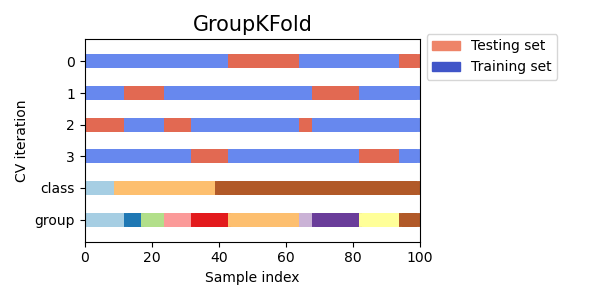
\includegraphics[width=0.75\linewidth]{Imagens/chap04/group_k_fold.png}
    \caption[Validação cruzada agrupada por regime]{Representação esquemática da validação cruzada agrupada por regime, implementada por meio do método \textit{GroupKFold}. Nesse procedimento, todas as observações pertencentes a um mesmo grupo experimental são mantidas na mesma partição, evitando que amostras correlacionadas sejam distribuídas simultaneamente entre treinamento e validação.}
    \fonte{\cite{sklearn_groupkfold_docs}.}
    \label{fig:groupkfold_validacao_metodologia}
\end{figure}

\section{Estratégia de Seleção de Modelos}
\label{sec:selecao_modelos}

A seleção de modelos neste trabalho foi estruturada de modo a considerar a organização das observações em regimes de operação e a comparação entre múltiplas famílias de modelos e combinações de hiperparâmetros. Como discutido na Fundamentação Teórica, quando muitos modelos são comparados a partir de estimativas de validação cruzada, a escolha baseada apenas no menor erro médio pode favorecer configurações que se destacam por flutuações amostrais, e não necessariamente por maior capacidade real de generalização.

Por esse motivo, a estratégia adotada não se limitou à seleção direta da configuração com menor erro médio de validação. Em vez disso, foi utilizado um procedimento hierárquico que combina três elementos principais: desempenho médio em validação cruzada, variabilidade do desempenho entre partições e parcimônia estrutural do modelo. Essa combinação busca tornar o processo de escolha mais robusto, evitando favorecer modelos excessivamente complexos quando sua vantagem de desempenho está dentro da variabilidade observada na validação.

Como definido na estratégia de validação, a métrica principal utilizada no processo de seleção foi o RMSE associado ao fluxo de permeado. Essa escolha permitiu orientar a seleção para a variável de maior interesse operacional e de maior complexidade preditiva aparente, mantendo as demais saídas no treinamento multissaída e na avaliação posterior de desempenho. Assim, a seleção foi conduzida com foco no fluxo, enquanto a análise final dos modelos considerou também a qualidade das predições das temperaturas de saída.

Dessa forma, a seleção de modelos foi conduzida em etapas sucessivas. Inicialmente, identificou-se o melhor desempenho médio em validação cruzada. Em seguida, definiu-se um conjunto de modelos candidatos dentro de uma margem de variabilidade em relação ao melhor modelo observado. Desse conjunto, selecionou-se a configuração de menor complexidade estrutural. Em caso de empate, o menor erro médio de validação foi utilizado como critério de desempate.

\subsection{Ferramentas Gráficas de Diagnóstico e Comparação dos Modelos}

Além das métricas numéricas obtidas por validação cruzada, o pipeline implementado gerou gráficos com finalidade diagnóstica e comparativa. Esses gráficos não substituem o critério formal de escolha adotado neste trabalho, mas complementam a análise ao permitir visualizar estabilidade, capacidade de generalização, comportamento do erro e qualidade preditiva para cada variável de interesse.

As principais ferramentas gráficas utilizadas são resumidas na Tabela~\ref{tab:graficos_diagnostico}.

\begin{table}[H]
\centering
\caption[Ferramentas gráficas utilizadas para diagnóstico dos modelos]{Ferramentas gráficas utilizadas para diagnóstico e comparação dos modelos ao longo do processo de seleção.}
\label{tab:graficos_diagnostico}
\begin{tabular}{p{4.3cm} p{9.5cm}}
\hline
\textbf{Gráfico} & \textbf{Finalidade} \\
\hline

Erro de validação cruzada versus complexidade
&
Avaliar o compromisso entre desempenho, variabilidade entre partições e parcimônia estrutural, evidenciando o melhor desempenho bruto, o limiar de seleção baseado em dispersão e a configuração selecionada. \\

Predito versus observado com predições \textit{out-of-fold} (OOF)
&
Avaliar a aderência entre valores previstos e valores experimentais para cada variável de saída, incluindo a reta identidade como referência visual. \\

RMSE por variável de saída
&
Comparar o desempenho dos modelos selecionados em cada parãmetro de desempenho, verificando se os ganhos se concentram no fluxo de permeado ou se também se refletem nas temperaturas de saída. \\

Curvas de aprendizagem
&
Acompanhar a evolução das perdas de treinamento e validação ao longo das épocas nos modelos neurais, auxiliando a interpretação do treinamento e do mecanismo de parada antecipada \\

Erro versus hiperparâmetro
&
Analisar a sensibilidade do modelo a um hiperparâmetro de interesse, permitindo identificar regiões de subajuste, bom compromisso entre ajuste e generalização, e possíveis sinais de sobreajuste. \\

\hline
\end{tabular}
\fonte{Elaborado pela autora.}
\end{table}

As predições \textit{out-of-fold} correspondem às previsões obtidas para cada observação quando essa observação pertence ao subconjunto de validação, isto é, quando não foi utilizada no ajuste do modelo naquela iteração. Dessa forma, os gráficos de valores preditos versus valores reais baseados em predições \textit{out-of-fold} OOF fornecem uma avaliação visual coerente com o procedimento de validação cruzada adotado.

\subsection{Critério Baseado em Um Desvio Padrão para Métricas de Erro}

Na Fundamentação Teórica, foi apresentada a regra clássica do \textit{one-standard-error}, baseada no erro padrão da média das métricas de validação. Na implementação computacional deste trabalho, entretanto, utilizou-se diretamente o atributo \texttt{std\_test\_score} fornecido pelo \texttt{GridSearchCV}, que corresponde ao desvio padrão da métrica de validação entre as partições da validação cruzada. Portanto, o critério aplicado corresponde a uma adaptação inspirada na lógica da regra \textit{one-standard-error}, mas baseada em um desvio padrão entre partições.

Seja

\begin{equation}
m^{\ast}=\arg\min_{m\in\mathcal{M}}\widehat{\mathcal{L}}^{CV}(m)
\label{eq:modelo_melhor_erro_medio}
\end{equation}

\noindent o modelo com menor erro médio estimado por validação cruzada. Para métricas de erro, define-se o limiar de seleção como

\begin{equation}
T=
\widehat{\mathcal{L}}^{CV}(m^{\ast})
+
\widehat{\sigma}^{CV}(m^{\ast}),
\label{eq:limiar_um_desvio}
\end{equation}

\noindent em que \(\widehat{\sigma}^{CV}(m^{\ast})\) representa o desvio padrão da métrica de validação entre as partições da validação cruzada para o modelo de menor erro médio.

O conjunto de modelos elegíveis segundo esse critério é dado por

\begin{equation}
\mathcal{C}=
\left\{
m\in\mathcal{M}:
\widehat{\mathcal{L}}^{CV}(m)\le T
\right\}.
\label{eq:conjunto_candidatos_um_desvio}
\end{equation}

Esse critério estabelece uma margem de tolerância em torno do melhor erro médio observado, considerando a variabilidade empírica das métricas de validação entre partições. Como utiliza o desvio padrão entre partições, e não o erro padrão da média, a margem adotada é mais ampla do que a regra clássica do \textit{one-standard-error}. Assim, o procedimento tende a favorecer a seleção de modelos mais parcimoniosos quando diferenças de desempenho estão dentro da variabilidade observada na validação cruzada.

\subsection{Critério Hierárquico de Seleção}

O critério hierárquico de seleção foi aplicado separadamente em cada busca de hiperparâmetros, isto é, dentro do conjunto de configurações candidatas pertencentes a uma mesma família de modelos. Dessa forma, nesta etapa, o objetivo não é comparar diretamente famílias distintas, mas selecionar, para cada família avaliada, a configuração de hiperparâmetros mais adequada segundo os critérios definidos.

Após a aplicação do critério baseado em um desvio padrão, obtém-se o conjunto \(\mathcal{C}\), composto pelas configurações candidatas cujo desempenho médio em validação cruzada se encontra dentro da margem de variabilidade em relação à melhor configuração observada. Em seguida, incorpora-se explicitamente um critério de parcimônia estrutural. Define-se inicialmente

\begin{equation}
C_{\min}=\min_{h\in\mathcal{C}} C(h),
\label{eq:complexidade_minima_configuracao}
\end{equation}

\noindent em que \(C(h)\) representa a medida de complexidade estrutural associada à configuração de hiperparâmetros \(h\).

Como a noção de complexidade depende da família de modelos considerada, foram adotadas medidas específicas para cada classe de modelo avaliada. Essas medidas são apresentadas na Tabela~\ref{tab:complexidade_modelos}.

Para os modelos lineares regularizados, essa medida foi definida em função do parâmetro de regularização \(\alpha\), que controla a intensidade da penalização aplicada aos coeficientes do modelo. Valores maiores de \(\alpha\) aumentam o peso da penalização e restringem mais fortemente os coeficientes, resultando em modelos efetivamente mais simples. Por outro lado, valores menores de \(\alpha\) reduzem a penalização e permitem maior liberdade de ajuste, sendo interpretados neste trabalho como configurações de maior complexidade efetiva. Por esse motivo, adotou-se a transformação \(-\log_{10}(\alpha)\) como proxy de complexidade para os modelos regularizados.

\begin{longtable}{p{4.2cm} p{9.8cm}}
\caption[Critérios de complexidade estrutural utilizados na seleção de configurações]{Critérios de complexidade estrutural utilizados na seleção de configurações de hiperparâmetros em cada família de modelos.}
\label{tab:complexidade_modelos}\\

\hline
\textbf{Família de modelos} & \textbf{Medida de complexidade adotada} \\
\hline
\endfirsthead

\hline
\textbf{Família de modelos} & \textbf{Medida de complexidade adotada} \\
\hline
\endhead

\hline
\multicolumn{2}{r}{\textit{Continua na próxima página}} \\
\endfoot

\hline
\endlastfoot

OLS &
Complexidade fixa, definida como \(C(h)=0\). \\

Ridge &
Complexidade definida por \(C(h)=-\log_{10}(\alpha)\). Menores valores de \(\alpha\) correspondem a maior complexidade efetiva. \\

Lasso e Lasso multissaída independente &
Complexidade definida por \(C(h)=-\log_{10}(\alpha)\). Na versão multissaída independente, aplica-se o mesmo critério ao estimador base. \\

ElasticNet e ElasticNet multissaída independente &
Complexidade definida por
\[
C(h)=-\log_{10}(\alpha)+0{,}01(1-l_1).
\]
O termo associado a \(l_1\) atua como ajuste secundário. \\

Árvore de decisão &
Complexidade definida principalmente pela profundidade máxima da árvore:
\[
C(h)=d-10^{-3}n_{\mathrm{leaf}},
\]
em que \(d=\texttt{max\_depth}\) e \(n_{\mathrm{leaf}}=\texttt{min\_samples\_leaf}\). Quando \(\texttt{max\_depth=None}\), atribui-se a \(d\) um valor elevado. \\

Random Forest &
Complexidade definida por
\[
C(h)=d+10^{-3}n_{\mathrm{est}}-10^{-6}n_{\mathrm{leaf}},
\]
em que \(d=\texttt{max\_depth}\), \(n_{\mathrm{est}}=\texttt{n\_estimators}\) e \(n_{\mathrm{leaf}}=\texttt{min\_samples\_leaf}\). \\

Gradient Boosting &
Complexidade definida por
\[
C(h)=d+10^{-3}n_{\mathrm{est}},
\]
em que \(d=\texttt{max\_depth}\) e \(n_{\mathrm{est}}=\texttt{n\_estimators}\). \\

MLP do \textit{scikit-learn} &
Complexidade aproximada por
\[
C(h)=\sum_{\ell=1}^{L} n_{\ell}+0{,}1L,
\]
em que \(n_{\ell}\) é o número de neurônios na camada \(\ell\) e \(L\) é o número de camadas ocultas. \\

MLP implementado em Keras e modelos neurais híbridos &
Complexidade aproximada por
\[
C(h)=\sum_{\ell=1}^{L} n_{\ell}+0{,}1L.
\]
Esse critério considera o número total de neurônios e o número de camadas ocultas. \\

\end{longtable}

Define-se então o subconjunto de configurações de menor complexidade como

\begin{equation}
\mathcal{C}_{\min}=
\left\{
h\in\mathcal{C}:
C(h)=C_{\min}
\right\}.
\label{eq:conjunto_complexidade_minima_configuracao}
\end{equation}

Caso múltiplas configurações apresentem a mesma complexidade mínima, utiliza-se o menor erro médio de validação entre elas como critério de desempate, selecionando-se

\begin{equation}
\widehat{h}=
\arg\min_{h\in\mathcal{C}_{\min}}
\widehat{\mathcal{L}}^{CV}(h).
\label{eq:configuracao_final_empate}
\end{equation}

A configuração \(\widehat{h}\) é então adotada como a configuração selecionada para a família de modelos considerada. Após a aplicação desse procedimento em cada família, os modelos resultantes, já com suas respectivas configurações selecionadas, são comparados entre si com base nas métricas de desempenho obtidas por validação cruzada. Dessa forma, o processo distingue duas etapas: primeiro, a seleção da configuração de hiperparâmetros dentro de cada família; depois, a comparação entre os modelos finais representantes de cada família.

\subsection{Comparação entre Famílias por Contagem de Parâmetros}

Enquanto a seleção dentro de cada família utilizou medidas de complexidade específicas para cada classe de modelo, a comparação entre famílias distintas empregou uma métrica universal: o número total de parâmetros treináveis de cada arquitetura. Essa abordagem permitiu posicionar modelos de naturezas fundamentalmente diferentes -- regressão linear, redes neurais e arquiteturas híbridas -- em uma mesma escala de complexidade.

O número de parâmetros de cada modelo foi calculado analiticamente a partir de sua arquitetura. Para a regressão linear (\texttt{OLS}), com cinco variáveis de entrada e três saídas, o total é de 18 parâmetros (15 coeficientes e 3 interceptos). Para as redes neurais e arquiteturas híbridas, a contagem depende do número de neurônios em cada camada, sendo a quantidade de parâmetros de uma camada densa dada por \(n_{\mathrm{in}} \times n_{\mathrm{out}} + n_{\mathrm{out}}\).

Como as buscas de hiperparâmetros foram conduzidas de forma independente para cada alvo, as arquiteturas selecionadas diferem entre si. Para os alvos \(T_{\mathrm{alim,out}}\) e \(T_{\mathrm{ref,out}}\), a configuração vencedora utiliza duas camadas ocultas com 128 e 64 neurônios e ativação \texttt{tanh}, totalizando 9219 parâmetros. Para o alvo \(Flux\), a configuração vencedora utiliza três camadas ocultas com 128, 64 e 32 neurônios e ativação \texttt{relu}, totalizando 11203 parâmetros.

Nas arquiteturas híbridas que utilizam todas as oito variáveis de entrada (cinco experimentais mais três predições físicas), como HPD e HRNN, a primeira camada recebe três entradas adicionais, acrescentando 384 parâmetros ao total. Dessa forma, para as baselines de \(T_{\mathrm{alim,out}}\) e \(T_{\mathrm{ref,out}}\), as arquiteturas HPD e HRNN totalizam 9603 parâmetros; para a baseline de \(Flux\), totalizam 11587 parâmetros. A arquitetura residual (ZohanResidual), embora receba as oito variáveis como entrada, aplica a rede neural apenas ao subconjunto de cinco variáveis experimentais e combina a saída por soma à predição física -- o que resulta na mesma contagem de parâmetros da baseline neural correspondente a cada alvo (9219 ou 11203, respectivamente).

Após o cálculo do número de parâmetros, aplicou-se novamente o critério baseado em um desvio padrão (1-SE), agora sobre o conjunto de todos os modelos candidatos de diferentes famílias. Entre os modelos dentro da margem de um desvio padrão do melhor desempenho, priorizou-se a arquitetura de menor número de parâmetros, retomando a lógica de parcimônia em uma escala comum de complexidade.

\begin{figure}[H]
    \centering
    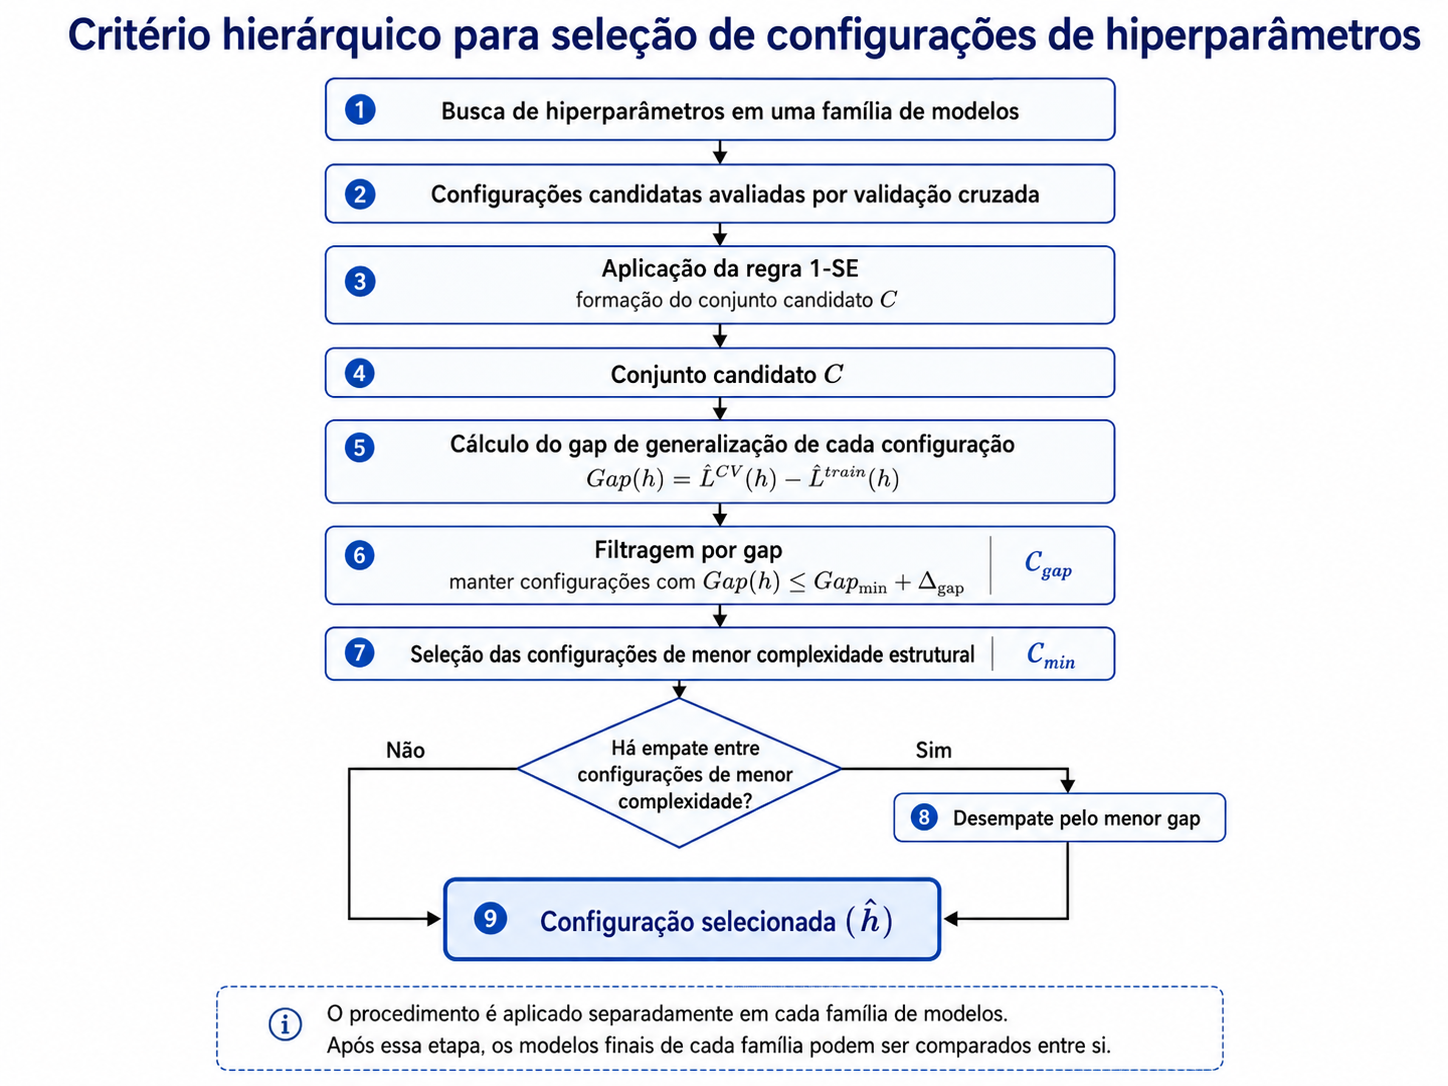
\includegraphics[width=1\linewidth]{Imagens/chap04/esquema_comp.png}
    \caption[Critério hierárquico de seleção de configurações]{Representação esquemática do critério hierárquico utilizado para selecionar a configuração de hiperparâmetros dentro de cada família de modelos. A partir do conjunto de configurações candidatas obtido após a aplicação do critério baseado em um desvio padrão, selecionam-se as configurações de menor complexidade estrutural e, em caso de empate, utiliza-se o menor erro médio de validação como critério final de desempate. Fonte: Elaborado pela Autora}

    \label{fig:criterio_hierarquico_selecao}
\end{figure}
\subsection{Implementação Computacional}

O procedimento foi implementado por meio do \texttt{GridSearchCV}, utilizando:

\begin{itemize}
    \item validação cruzada baseada em \textit{GroupKFold};
    \item encapsulamento das etapas de pré-processamento e modelagem em \textit{Pipeline}, garantindo que transformações dependentes dos dados, como a padronização, fossem ajustadas apenas no subconjunto de treinamento de cada partição;
    \item cálculo simultâneo dos erros de treinamento e validação, por meio de \texttt{return\_train\_score=True};
    \item função personalizada de \texttt{refit}, responsável por implementar o critério baseado em um desvio padrão, seguido da minimização da complexidade estrutural e do desempate final pelo menor erro de validação.
\end{itemize}

A utilização direta das estatísticas disponíveis em \texttt{cv\_results\_}, como \texttt{mean\_test\_score}, \texttt{std\_test\_score}, permitiu integrar avaliação de desempenho, variabilidade entre partições e parcimônia estrutural em um único procedimento de seleção calibrada.
\section{Estrutura Computacional da Comparação entre Modelos}

A implementação computacional do procedimento de modelagem foi estruturada como um pipeline unificado de comparação entre famílias de modelos. Esse pipeline integra as etapas de pré-processamento, busca de hiperparâmetros, validação cruzada e seleção final de modelos em um fluxo reprodutível.

O objetivo dessa organização é garantir que todas as famílias avaliadas sejam submetidas ao mesmo protocolo de avaliação, permitindo comparações consistentes de desempenho e evitando diferenças artificiais decorrentes de procedimentos distintos de treinamento ou validação.

\subsection{Organização geral do pipeline}

O processo de modelagem foi estruturado em três etapas principais, mantendo-se, em todas elas, o mesmo protocolo geral de avaliação: validação cruzada agrupada por \textit{Regime}, cálculo das métricas de desempenho em treino e validação e seleção de configurações com base no critério hierárquico descrito anteriormente. As diferenças entre as etapas dizem respeito principalmente às famílias de modelos avaliadas e à extensão da busca de hiperparâmetros realizada.

Na primeira etapa, foram avaliados modelos clássicos de regressão supervisionada, incluindo modelos lineares, modelos lineares regularizados e modelos baseados em árvores. Para essas famílias, a busca de hiperparâmetros foi conduzida por meio de \texttt{GridSearchCV}, utilizando validação cruzada baseada em \textit{GroupKFold}. Nos modelos sensíveis à escala das variáveis, as etapas de pré-processamento foram encapsuladas em \textit{Pipeline}, garantindo que a padronização das variáveis de entrada fosse ajustada apenas sobre os dados de treinamento de cada partição.

Na segunda etapa, foram avaliadas redes neurais do tipo \textit{Multi-Layer Perceptron}. Também nessa etapa, a seleção de configurações foi realizada por meio de \texttt{GridSearchCV} associado ao \textit{GroupKFold}, permitindo comparar diferentes arquiteturas sob o mesmo procedimento de validação adotado para os demais modelos. Devido ao maior custo computacional associado ao treinamento dessas arquiteturas, a busca foi limitada a grades previamente definidas de hiperparâmetros, contemplando combinações de tamanho da rede, regularização e parâmetros de treinamento.

Na terceira etapa, foram investigadas estratégias híbridas que integram estimativas provenientes do modelo físico reduzido ao processo de aprendizado das redes neurais, conforme descrito na Seção~\ref{sec:modelos-hibridos}. Nessa fase, a busca de hiperparâmetros foi restringida a arquiteturas previamente identificadas como competitivas, reduzindo o espaço de busca e o custo computacional total. Assim como nas etapas anteriores, a avaliação foi conduzida por validação cruzada agrupada, preservando a separação por \textit{Regime}.

Essa estrutura sequencial permite comparar famílias de modelos sob um procedimento de avaliação comum, ao mesmo tempo em que controla o custo computacional da análise. A organização em etapas também possibilita verificar, de forma progressiva, se o aumento de complexidade estrutural — de modelos clássicos para redes neurais e, posteriormente, para abordagens híbridas — resulta em ganhos efetivos de desempenho preditivo.
\subsection{Estratégias de redução de custo computacional}

O treinamento de modelos de aprendizado de máquina, particularmente redes neurais, pode envolver elevado custo computacional quando múltiplas combinações de hiperparâmetros são avaliadas sob validação cruzada. Para tornar o processo viável, foram adotadas estratégias específicas de otimização do treinamento.

Para os modelos neurais implementados em \texttt{Keras}, utilizou-se o mecanismo de parada antecipada (do inglês, \textit{early stopping}, no qual o treinamento é interrompido automaticamente quando a perda de validação deixa de apresentar melhora significativa após um número predefinido de épocas. Essa estratégia evita treinamento desnecessário após a convergência do modelo.

Adicionalmente, empregou-se o mecanismo de redução adaptativa da taxa de aprendizado (\textit{learning rate scheduling}), no qual a taxa de aprendizado é automaticamente reduzida quando o desempenho de validação permanece estagnado por um determinado número de épocas. Essa estratégia permite refinar o processo de otimização próximo ao mínimo da função de perda.

Também foi utilizado um mecanismo de interrupção automática em caso de instabilidade numérica (\texttt{TerminateOnNaN}), garantindo robustez durante o treinamento.

Essas estratégias combinadas permitem reduzir significativamente o tempo total de treinamento sem comprometer a qualidade das soluções encontradas.

\subsection{Geração automática de análises gráficas}

Além das métricas numéricas obtidas na validação cruzada, o pipeline foi estruturado para gerar automaticamente um conjunto de análises gráficas utilizadas na interpretação dos resultados.

Entre os artefatos gráficos produzidos estão:

\begin{itemize}
\item gráficos de desempenho em função da complexidade estrutural dos modelos;
\item gráficos de valores previstos versus valores experimentais obtidos a partir de predições \textit{out-of-fold};
\item curvas de treinamento e validação para as arquiteturas neurais;
\item análises de sensibilidade local do erro em relação aos hiperparâmetros principais;
\item gráficos comparativos de desempenho entre modelos para cada variável-alvo.
\end{itemize}

Essas representações visuais auxiliam na interpretação do comportamento dos modelos, permitindo identificar tendências de sobreajuste, regimes de complexidade adequada e diferenças de desempenho entre famílias de modelos.

\subsection{Avaliação Final por Predições \textit{Out-of-Fold} (OOF)}
\label{sec:avaliacao_oof}

Conforme discutido na Seção~\ref{sec:selecao_modelos}, o critério hierárquico de seleção utiliza o erro médio de validação cruzada (CV RMSE) para comparar e escolher a configuração de hiperparâmetros de cada família. No entanto, essa estimativa pode apresentar viés otimista, uma vez que o mesmo conjunto de validação cruzada é empregado tanto para selecionar a configuração quanto para estimar seu desempenho, favorecendo configurações que se destacam por flutuações amostrais (\cite{Cawley2010Overfitting}).

Para obter uma estimativa menos tendenciosa do desempenho preditivo, adotou-se um procedimento de predições \textit{out-of-fold} (OOF). Após a seleção da configuração ótima, um novo modelo é instanciado com os hiperparâmetros escolhidos e retreinado independentemente em cada partição da validação cruzada, partindo de uma nova inicialização aleatória. As predições sobre as amostras mantidas fora do treinamento em cada partição são então concatenadas, formando um conjunto completo de predições. Diferentemente da função \texttt{cross\_val\_predict} do \textit{scikit-learn}, que retorna predições obtidas durante o próprio processo de validação cruzada e não é recomendada como medida de erro de generalização (\cite{sklearn_cv_docs}), o procedimento aqui adotado realiza um re-treinamento independente do modelo selecionado em cada partição, produzindo uma estimativa de desempenho posterior ao processo de seleção.

As métricas finais de desempenho reportadas neste trabalho (RMSE OOF e R$^2$ OOF) são calculadas sobre essas predições concatenadas, garantindo que cada amostra seja prevista por um modelo que não a utilizou durante o treinamento.

\section{Famílias de Modelos Avaliadas}

A seleção das famílias de modelos avaliadas neste trabalho foi conduzida com o objetivo de comparar abordagens de regressão supervisionada com diferentes níveis de flexibilidade estrutural, interpretabilidade e capacidade de representação. Como o conjunto de dados envolve variáveis operacionais contínuas e múltiplas variáveis de saída, buscou-se avaliar desde modelos mais simples e parcimoniosos até métodos com maior capacidade de capturar relações não lineares entre as entradas e as respostas do sistema.


Dessa forma, a comparação entre famílias de modelos permite investigar empiricamente a adequabilidade dos modelos lineares como referência de baixa complexidade, verificando se formulações mais simples são capazes de representar satisfatoriamente a relação entre as variáveis operacionais e as respostas do sistema. Além disso, possibilita avaliar o ganho de desempenho associado à inclusão de modelos não lineares, por meio da comparação entre modelos lineares, modelos baseados em árvores e redes neurais sob o mesmo protocolo de validação cruzada. Essa análise também permite examinar o efeito do aumento de flexibilidade estrutural sobre a capacidade de generalização, considerando conjuntamente o erro de validação e a complexidade estrutural. Por fim, a comparação entre famílias fornece subsídios para avaliar o compromisso entre desempenho preditivo, estabilidade entre partições e parcimônia, levando em conta as métricas médias de validação cruzada, a variabilidade entre partições e a complexidade da configuração selecionada em cada família de modelos.

\subsection{Modelos Lineares}

Os modelos lineares (OLS, Ridge, Lasso, Elastic Net e variantes multi-task) representam a classe de menor flexibilidade estrutural considerada neste trabalho.

Sua inclusão é justificada por três razões principais:

\begin{enumerate}
    \item Servem como modelo de referência (\emph{baseline}), permitindo quantificar o ganho obtido com o aumento de flexibilidade estrutural;
    \item São consistentes com a hipótese de comportamento aproximadamente afim das temperaturas de saída;
    \item Permitem controle explícito da complexidade via regularização, favorecendo estabilidade em cenários com número limitado de observações.
\end{enumerate}

As variantes regularizadas possibilitam investigar o impacto da penalização sobre o compromisso viés--variância, sendo particularmente relevantes quando há potencial multicolinearidade entre variáveis operacionais.

\subsection{Modelos Baseados em Árvores}

Os modelos baseados em árvores, incluindo Árvore de Decisão, Random Forest e Gradient Boosting, introduzem flexibilidade não linear por meio de particionamentos sucessivos do espaço de atributos. A partir desses particionamentos, tais modelos conseguem representar relações não lineares e interações entre variáveis de entrada sem que essas relações precisem ser especificadas previamente na formulação do modelo. Dessa forma, a estrutura do modelo é construída de maneira orientada pelos padrões observados nos dados, permitindo que diferentes regiões do espaço de entrada sejam associadas a comportamentos distintos das variáveis de saída.

A inclusão dessa família permite avaliar se métodos não lineares baseados em particionamento do espaço de entrada oferecem ganhos consistentes de desempenho em relação aos modelos lineares, mantendo um nível intermediário de complexidade estrutural. A Árvore de Decisão fornece uma representação mais simples e interpretável, enquanto os métodos de ensemble, como Random Forest e Gradient Boosting, ampliam a capacidade preditiva ao combinar múltiplas árvores. No caso do Random Forest, essa combinação contribui para reduzir a variância associada a árvores individuais; já no Gradient Boosting, as árvores são ajustadas de forma sequencial, buscando corrigir os erros residuais dos modelos anteriores.
\subsection{Redes Neurais}

As redes neurais do tipo Multi-Layer Perceptron (MLP) representam a classe de maior flexibilidade estrutural considerada.

Como aproximadores universais de funções contínuas, são capazes de modelar relações altamente não lineares e interações complexas entre variáveis. Sua inclusão tem dois objetivos principais:

\begin{enumerate}
    \item Avaliar se o aumento substancial de capacidade representacional produz ganhos significativos de desempenho no domínio experimental considerado.
    \item Investigar o limite superior de flexibilidade necessário para capturar o comportamento conjunto das variáveis-alvo.
\end{enumerate}

Ao incluir redes neurais na comparação, torna-se possível verificar se a estrutura física subjacente pode ser adequadamente representada por modelos de complexidade moderada ou se demanda representações mais expressivas.

\subsection{Comparação entre Níveis de Flexibilidade Estrutural}

A seleção dessas três famílias estabelece um espectro crescente de flexibilidade estrutural:

\begin{center}
Modelos Lineares $\rightarrow$ Árvores $\rightarrow$ Redes Neurais
\end{center}

Essa organização permite confrontar as hipóteses físicas iniciais com evidências empíricas obtidas sob validação cruzada estruturada por grupos experimentais, mantendo coerência entre fundamentação física e estratégia estatística de modelagem.
\section{Tuning de Hiperparâmetros}
\label{sec:tuning}

O procedimento de \textit{tuning} tem como objetivo explorar o espaço de hiperparâmetros $\Theta_{\mathcal{F}}$ de cada família de modelos, gerando o conjunto de configurações candidatas que posteriormente serão avaliadas segundo a estratégia hierárquica de seleção descrita na Seção~4.4. Assim, o \textit{tuning} não constitui, por si só, o critério final de escolha, mas sim a etapa de geração sistemática de alternativas estruturais dentro de cada família considerada.

\subsubsection{Procedimento de busca e validação}

A busca de hiperparâmetros foi conduzida conforme o protocolo de validação descrito na Seção~\ref{sec:validacao_cruzada}, utilizando validação cruzada agrupada por \textit{Regime}. Dessa forma, todas as configurações avaliadas foram comparadas sob a mesma estrutura de particionamento, preservando a separação entre regimes experimentais durante o treinamento e a validação.

Para todas as famílias avaliadas, as etapas de pré-processamento e modelagem foram organizadas em uma estrutura única de execução, de modo que as transformações dependentes dos dados fossem ajustadas apenas no subconjunto de treinamento de cada partição. Em particular, a padronização das variáveis de entrada foi realizada por meio do procedimento de média zero e variância unitária, conforme descrito anteriormente. Além disso, em algumas famílias de modelos foi utilizado um procedimento análogo para escalonamento das variáveis de saída, permitindo que o treinamento fosse realizado no espaço padronizado das variáveis-alvo e que as predições fossem posteriormente convertidas para a escala física original.

Embora os modelos tenham sido treinados para prever simultaneamente as três variáveis de saída consideradas, o processo de seleção de hiperparâmetros foi orientado prioritariamente pelo desempenho associado ao fluxo de permeado. Essa definição é coerente com a estratégia metodológica adotada, na qual o fluxo foi tratado como a variável crítica de seleção por representar diretamente a produtividade do sistema e por apresentar maior complexidade preditiva aparente nas análises preliminares.

Para implementar esse critério, utilizou-se uma função de pontuação personalizada baseada no RMSE da variável de fluxo. Como o procedimento computacional de busca de hiperparâmetros realiza a maximização da função de pontuação, essa métrica foi implementada como o negativo do RMSE, de modo que maximizar a pontuação equivale, na prática, a minimizar o erro associado ao fluxo de permeado. As demais variáveis de saída foram mantidas no treinamento multissaída e avaliadas posteriormente, permitindo verificar se a priorização do fluxo preservava a capacidade do modelo de predizer adequadamente as temperaturas de saída do sistema.

Para isso, utilizou-se uma função de pontuação personalizada baseada no RMSE da variável de fluxo. Como o procedimento computacional de busca de hiperparâmetros realiza a maximização da função de pontuação, essa métrica foi implementada como o negativo do RMSE, de modo que maximizar a pontuação equivale, na prática, a minimizar o erro associado ao fluxo de permeado. Ainda assim, as demais variáveis de saída foram mantidas no treinamento e avaliadas posteriormente, permitindo verificar se a priorização do fluxo não comprometia de forma significativa a predição das temperaturas de saída.


\subsection{Espaços de busca por família}
\label{subsec:espacos_busca}

Os espaços de busca foram definidos de modo a abranger diferentes níveis de flexibilidade estrutural dentro de cada família de modelos, mantendo coerência com a definição operacional de complexidade adotada neste trabalho. Nas regressões regularizadas, o parâmetro \(\alpha\) controla a intensidade da penalização aplicada aos coeficientes: valores maiores de \(\alpha\) impõem maior regularização, enquanto valores menores reduzem esse efeito. No caso do Elastic Net, o parâmetro \(l_1\text{-ratio}\) controla a combinação entre as penalizações \(L_1\) e \(L_2\).

\begin{longtable}{p{3.8cm} p{9.8cm}}
\caption[Espaços de busca de hiperparâmetros por família de modelos]{Espaços de busca de hiperparâmetros avaliados para cada família de modelos.}
\label{tab:espacos_busca_modelos}\\

\hline
\textbf{Família/modelo} & \textbf{Espaço de busca avaliado} \\
\hline
\endfirsthead

\hline
\textbf{Família/modelo} & \textbf{Espaço de busca avaliado} \\
\hline
\endhead

\hline
\multicolumn{2}{r}{\textit{Continua na próxima página}} \\
\endfoot

\hline
\endlastfoot

OLS
&
Sem hiperparâmetros. Utilizado como referência linear sem regularização. \\

Ridge
&
\(\alpha \in \{10^{-3},10^{-2},10^{-1},1,10,100\}\). \\

Lasso MultiTask
&
\(\alpha \in \{10^{-4},10^{-3},10^{-2},10^{-1},1\}\). \\

ElasticNet MultiTask
&
\(\alpha \in \{10^{-4},10^{-3},10^{-2},10^{-1},1\}\);
\(l_1\text{-ratio} \in \{0{,}1,0{,}3,0{,}5,0{,}7,0{,}9\}\). \\

Lasso independente multissaída
&
\(\alpha \in \{10^{-4},10^{-3},10^{-2},10^{-1},1\}\). Implementado por meio de estimadores independentes para cada saída. \\

ElasticNet independente multissaída
&
\(\alpha \in \{10^{-4},10^{-3},10^{-2},10^{-1},1\}\);
\(l_1\text{-ratio} \in \{0{,}1,0{,}3,0{,}5,0{,}7,0{,}9\}\). Implementado por meio de estimadores independentes para cada saída. \\

Árvore de decisão
&
\(\texttt{max\_depth} \in \{2,3,4,5,6,\texttt{None}\}\);
\(\texttt{min\_samples\_leaf} \in \{1,2,5,8,10\}\);
\(\texttt{min\_samples\_split} \in \{2,5,10,15\}\);
\(\texttt{ccp\_alpha} \in \{0,10^{-4},10^{-3},10^{-2}\}\). \\

Random Forest
&
\(\texttt{n\_estimators} \in \{200,400,600\}\);
\(\texttt{max\_depth} \in \{2,3,4,5,\texttt{None}\}\);
\(\texttt{min\_samples\_leaf} \in \{1,2,5,8,10\}\);
\(\texttt{min\_samples\_split} \in \{2,5,10\}\);
\(\texttt{max\_features} \in \{0{,}5,0{,}8,1{,}0\}\). \\

Gradient Boosting
&
\(\texttt{n\_estimators} \in \{50,100,200,400\}\);
\(\texttt{learning\_rate} \in \{0{,}01,0{,}03,0{,}05,0{,}1\}\);
\(\texttt{max\_depth} \in \{1,2,3\}\);
\(\texttt{min\_samples\_leaf} \in \{1,2,5,10\}\);
\(\texttt{subsample} \in \{0{,}6,0{,}8,1{,}0\}\).
Utilizou-se modelagem independente para viabilizar a predição multissaída. \\

MLP no \textit{scikit-learn}
&
\(\texttt{hidden\_layer\_sizes} \in \{(32,), (64,), (64,32), (128,64)\}\);
\(\alpha \in \{0,10^{-6},10^{-5},10^{-4}\}\);
\(\texttt{learning\_rate\_init} \in \{3\times10^{-3},10^{-3},3\times10^{-4},10^{-4}\}\). \\

KerasMLP baseline
&
\(\texttt{hidden\_layer\_sizes} \in \{(32,), (64,), (128,), (256,), (64,32), (128,64), (256,128), (128,64,32), (256,128,64)\}\);
\(\texttt{learning\_rate} \in \{10^{-3},3\times10^{-4}\}\);
\(\texttt{l2} \in \{0,10^{-6},10^{-5}\}\).
Foram mantidos fixos: ativação ReLU, otimizador Adam, função de perda Huber, \(\delta=1{,}0\), lote de 64 amostras, 200 épocas e fração de validação interna de 0,2. \\

KerasMLP FrozenBaseline
&
Utiliza diretamente a configuração baseline selecionada, sem variação adicional relevante de hiperparâmetros. Atua como referência neural não híbrida. \\

KerasMLP Luc Restricted
&
Mantém a estrutura da baseline e varia os hiperparâmetros associados ao termo físico na função de perda:
\(\texttt{physics\_norm} \in \{\texttt{mse},\texttt{mae}\}\);
\(\omega \in \{0{,}0,0{,}1,0{,}3,0{,}5,0{,}7\}\). \\

KerasMLP ZohanHPD Restricted
&
Utiliza como entrada o vetor experimental concatenado às predições físicas. A busca é restrita a uma vizinhança do parâmetro \(l_2\):
\(\texttt{l2} \in \{\texttt{l2}_{base},0,10^{-6},10^{-5},10^{-4}\}\). \\

KerasMLP ZohanResidual Restricted
&
Adota arquitetura residual baseada na soma entre a predição física e uma correção aprendida. A busca é restrita a uma vizinhança do parâmetro \(l_2\):
\(\texttt{l2} \in \{\texttt{l2}_{base},0,10^{-6},10^{-5},10^{-4}\}\). \\

KerasMLP ZohanHRNN Restricted
&
Combina entrada expandida com correção residual, mantendo a configuração baseline como referência. A busca é restrita ao parâmetro \(l_2\):
\(\texttt{l2} \in \{\texttt{l2}_{base},0,10^{-6},10^{-5},10^{-4}\}\). \\

\end{longtable}

A organização em tabela permite explicitar, de forma compacta, quais hiperparâmetros foram efetivamente explorados em cada família. Nos modelos lineares regularizados, a busca concentra-se principalmente na intensidade da penalização. Nos modelos baseados em árvores, os hiperparâmetros controlam a profundidade, o número de estimadores e o tamanho mínimo das partições. Nas redes neurais, a busca envolve principalmente arquitetura, taxa de aprendizado e regularização. Já nas famílias híbridas, a busca foi restringida a hiperparâmetros específicos, mantendo como referência a configuração neural baseline previamente selecionada.

\section{Uso do Modelo Físico na Estratégia de Modelagem}

O modelo físico reduzido do módulo de dessalinização, previamente descrito na Fundamentação Teórica, não constitui o objeto de desenvolvimento deste trabalho, mas é empregado como elemento auxiliar na estratégia de modelagem supervisionada proposta.

\subsection{Papel Metodológico}

Neste estudo, o modelo físico desempenha duas funções principais: (i) atuar como referência comparativa para avaliação do desempenho dos modelos orientados a dados e (ii) integrar estratégias híbridas de aprendizado, nas quais informações físicas são incorporadas ao processo de treinamento das redes neurais.

Dessa forma, o modelo físico fornece uma base interpretativa fundamentada em princípios de conservação e termodinâmicos, permitindo analisar em que medida abordagens puramente orientadas a dados são capazes de reproduzir, corrigir ou superar seu desempenho preditivo.

\subsection{Integração Híbrida e Comparação com Modelos Baseados em Dados}

Nas estratégias híbridas avaliadas, o modelo físico é utilizado não apenas como referência comparativa, mas também como fonte de conhecimento adicional incorporado ao processo de aprendizado dos modelos baseados em dados.

A integração entre conhecimento físico e aprendizado de máquina pode ser realizada de diferentes formas, dependendo da maneira como a informação proveniente do modelo físico é utilizada durante o treinamento. Neste trabalho, foram investigadas diferentes estratégias de integração físico--dados, tomando o modelo físico reduzido como fonte de informação estruturada para auxiliar o aprendizado supervisionado.

Além das arquiteturas híbridas propriamente ditas, a comparação incluiu também uma rede neural baseline com hiperparâmetros congelados, utilizada como referência para avaliar em que medida a incorporação explícita de informação física produz ganhos efetivos de desempenho.

\subsection{Estratégias de Integração Físico--Dados}

Com o objetivo de avaliar diferentes formas de incorporar conhecimento físico ao processo de aprendizado, foram implementadas quatro estratégias de modelagem híbrida físico--dados. Essas estratégias diferem quanto ao papel atribuído à predição do modelo físico reduzido: ela pode ser utilizada como variável adicional de entrada, como aproximação inicial a ser corrigida pela rede neural, como componente simultâneo de entrada e correção residual, ou ainda como termo auxiliar na função de perda.

Em particular, as três primeiras estratégias seguem formas de integração discutidas na literatura de \textit{physics-informed machine learning}, nas quais o modelo físico pode atuar como fonte adicional de informação, como referência inicial para uma correção residual ou como parte da arquitetura híbrida da rede \cite{zhou2025physics}. A Figura~\ref{fig:hrnn_model} apresenta essas três arquiteturas de forma esquemática, servindo como referência visual para as subseções seguintes. A estrutura (A) corresponde ao modelo \textit{Hybrid Physics Data} (HPD), em que a predição física é concatenada às variáveis experimentais de entrada. A estrutura (B) corresponde ao modelo residual, no qual a rede neural aprende uma correção a ser somada à predição física. Por fim, a estrutura (C) corresponde ao modelo \textit{Hybrid Residual Neural Network} (HRNN), que combina simultaneamente a entrada física auxiliar e a correção residual.

\begin{figure}[H]
\centering
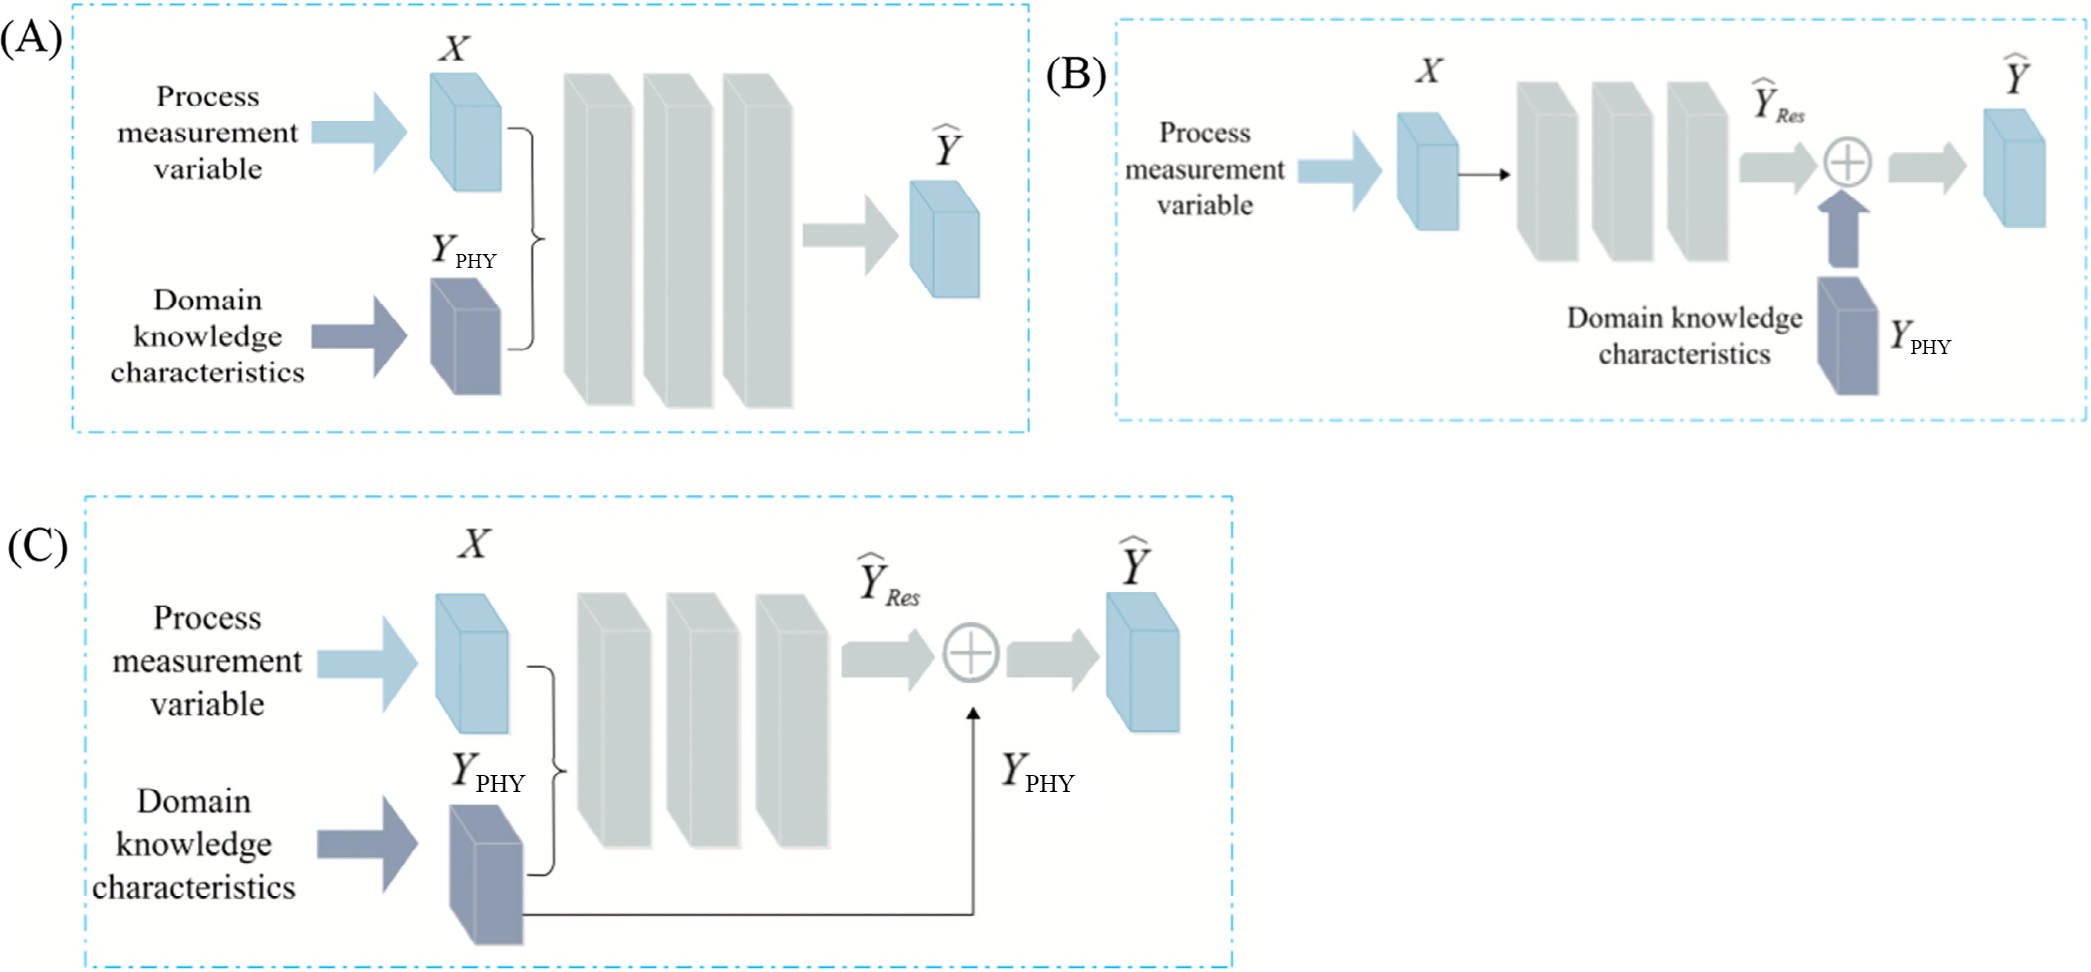
\includegraphics[width=1.0\textwidth]{Imagens/chap04/hybrids.png}
\caption[Estratégias híbridas físico--dados implementadas no trabalho]{Representação esquemática das estratégias híbridas físico--dados implementadas neste trabalho. As estruturas (A), (B) e (C) correspondem, respectivamente, ao modelo \textit{Hybrid Physics Data} (HPD), ao modelo residual e ao modelo \textit{Hybrid Residual Neural Network} (HRNN). Em (A), a predição do modelo físico é utilizada como entrada adicional da rede neural; em (B), a rede aprende um termo residual somado à predição física; e, em (C), essas duas estratégias são combinadas em uma única arquitetura. Fonte: adaptado de \cite{zhou2025physics}.}
\label{fig:hrnn_model}
\end{figure}

\subsubsection{Modelo Híbrido com Predições Físicas como Variáveis de Entrada (HPD)}

A primeira estratégia consiste em utilizar diretamente as predições do modelo físico reduzido como variáveis adicionais de entrada da rede neural. Essa abordagem corresponde ao modelo híbrido \textit{Hybrid Physics Data} (HPD), representado esquematicamente na Figura~\ref{fig:hrnn_model}(A) \cite{zhou2025physics}.

Se \(\mathbf{X}\) representa o vetor de variáveis experimentais de entrada e \(Y_{\text{PHY}}\) representa a predição fornecida pelo modelo físico, o vetor de entrada expandido pode ser definido como

\begin{equation}
\mathbf{X}' = [\mathbf{X}, Y_{\text{PHY}}].
\end{equation}

Dessa forma, a rede neural recebe simultaneamente informações provenientes das condições operacionais medidas e das estimativas produzidas pelo modelo físico. A função da rede, nesse caso, é aprender a relação entre esse conjunto expandido de entradas e as respostas experimentais, podendo explorar complementaridades entre as variáveis medidas e a aproximação física disponível.

\subsubsection{Modelagem Residual Baseada no Modelo Físico}

A segunda estratégia consiste em utilizar o modelo físico como uma aproximação inicial do sistema e treinar a rede neural para aprender uma correção residual. Essa formulação corresponde à estrutura representada na Figura~\ref{fig:hrnn_model}(B), associada à modelagem híbrida residual \cite{zhou2025physics}.

Seja \(Y_{\text{PHY}}\) a predição fornecida pelo modelo físico e \(Y\) o valor experimental observado. Conceitualmente, o resíduo associado ao modelo físico pode ser definido como

\begin{equation}
Y_{\text{res}} = Y - Y_{\text{PHY}}.
\end{equation}

Na implementação adotada neste trabalho, a rede neural não foi treinada a partir de um conjunto-alvo residual explicitamente separado. Em vez disso, a arquitetura foi construída de modo que sua saída representasse diretamente uma correção aprendida sobre a predição física. Assim, a predição final do modelo assume a forma

\begin{equation}
\hat{Y} = Y_{\text{PHY}} + \hat{Y}_{\text{res}},
\end{equation}

\noindent em que \(\hat{Y}_{\text{res}}\) corresponde ao termo corretivo produzido pela rede neural. Nessa abordagem, o modelo físico fornece uma estimativa inicial, enquanto a rede neural aprende a compensar desvios sistemáticos em relação aos dados experimentais.

\subsubsection{Hybrid Residual Neural Network (HRNN)}

A terceira estratégia combina as duas abordagens anteriores em uma única arquitetura, denominada \textit{Hybrid Residual Neural Network} (HRNN). Essa formulação corresponde à estrutura representada na Figura~\ref{fig:hrnn_model}(C) \cite{zhou2025physics}.

Nesse caso, a rede neural utiliza simultaneamente as variáveis experimentais e a predição do modelo físico como entradas, ao mesmo tempo em que produz uma correção residual somada à estimativa física. Portanto, diferentemente do HPD, em que a predição física atua apenas como variável adicional de entrada, e do modelo residual, em que a rede aprende apenas a correção sobre a estimativa física, o HRNN integra os dois mecanismos na mesma arquitetura.

Matematicamente, a predição final pode ser representada por

\begin{equation}
\hat{Y} = f_{NN}(X, Y_{\text{PHY}}) + Y_{\text{PHY}},
\end{equation}

\noindent em que \(f_{NN}(X, Y_{\text{PHY}})\) representa o termo corretivo aprendido pela rede a partir das variáveis experimentais e das predições do modelo físico.

Nesse contexto, o modelo físico fornece uma aproximação inicial do comportamento do sistema, enquanto a rede neural aprende a corrigir vieses sistemáticos e desvios estruturais em relação aos dados experimentais. Dessa forma, o HRNN busca combinar a informação fenomenológica fornecida pelo modelo reduzido com a flexibilidade de representação da rede neural.

\subsubsection{Regularização da Função de Perda com Predições do Modelo Físico}

A quarta estratégia de integração físico--dados consiste em incorporar diretamente as predições do modelo físico à função de perda utilizada no treinamento da rede neural. Diferentemente das três arquiteturas apresentadas na Figura~\ref{fig:hrnn_model}, essa abordagem não altera necessariamente o vetor de entrada ou a forma da predição final, mas modifica o critério de treinamento da rede ao incluir uma penalização associada à discrepância em relação ao modelo físico. Essa estratégia foi explorada por \cite{seixo2024internship} no contexto da modelagem de sistemas de destilação por membranas.

Nessa formulação, além do termo de ajuste aos dados experimentais, inclui-se um termo adicional que penaliza a diferença entre a predição da rede e a predição física. De forma geral, a função objetivo pode ser escrita como

\begin{equation}
\mathcal{L} = (1-\omega)\mathcal{L}_{t} + \omega \mathcal{L}_{\Phi},
\end{equation}

\noindent em que \(\omega \in [0,1]\) controla o peso relativo atribuído ao termo físico. Quando \(\omega = 0\), o treinamento é guiado apenas pelo ajuste aos dados experimentais; à medida que \(\omega\) aumenta, cresce a influência da concordância com o modelo físico na função objetivo.

O termo de ajuste aos dados experimentais pode ser representado por

\begin{equation}
\mathcal{L}_{t} = H_{\delta}(y_{\text{true}} - y_{\text{pred}}),
\end{equation}

\noindent em que \(H_{\delta}\) representa a perda de Huber. Já o termo físico corresponde a uma medida de discrepância entre a predição da rede e a predição do modelo físico, podendo assumir forma quadrática média ou erro absoluto médio, a depender da configuração avaliada:

\begin{equation}
\mathcal{L}_{\Phi} = D(y_{\text{model}}, y_{\text{pred}}).
\end{equation}

Na implementação utilizada neste trabalho, foram avaliadas diferentes escolhas para \(D(\cdot,\cdot)\), em particular normas do tipo MSE e MAE, de modo a investigar o efeito da forma do termo físico sobre o treinamento. Essa estratégia permite avaliar se a aproximação física pode atuar como regularização auxiliar, orientando a rede neural para soluções mais coerentes com o modelo fenomenológico disponível.
\subsection{Limitações da Integração}

Por se tratar de um modelo reduzido, o modelo físico empregado incorpora simplificações estruturais que limitam sua capacidade de representar integralmente os fenômenos presentes no sistema experimental real. Assim, sua incorporação às arquiteturas híbridas foi conduzida de forma controlada e sempre avaliada de modo comparativo em relação a modelos puramente orientados a dados.

Além disso, embora a informação física seja utilizada de diferentes maneiras nas estratégias híbridas, a seleção de hiperparâmetros em todas as famílias permaneceu orientada prioritariamente pelo desempenho preditivo sobre o fluxo de permeado, variável adotada neste trabalho como principal indicador de produtividade do sistema V-AGMD. Dessa forma, o impacto da integração físico--dados foi avaliado não apenas sob o ponto de vista conceitual, mas também em termos de sua contribuição efetiva para a generalização no alvo de maior interesse do estudo.
